\documentclass[12pt,a4paper]{article}
\usepackage{pdfpages}
\usepackage[T1]{fontenc}
\usepackage{lmodern} % <-- Agrega esta línea
\usepackage{float} % Permite usar la opción [H] para fijar figuras
\usepackage[utf8]{inputenc}
\usepackage[spanish,es-tabla]{babel}
\usepackage{geometry}
\usepackage{graphicx}
\usepackage[table]{xcolor}
\usepackage{tcolorbox}
\tcbuselibrary{breakable}
\usepackage{microtype}
\usepackage{caption}
\usepackage{subcaption}
\usepackage{fancyhdr}
\usepackage{amsmath}
\usepackage{parskip}
\usepackage{booktabs}
\usepackage{array}
\usepackage{siunitx}
\usepackage{float}
\usepackage{enumitem}
\usepackage{hyperref}

% ==============================================================================
% CONFIGURACIONES GLOBALES Y COMANDOS PERSONALIZADOS
% ==============================================================================

% Configuración de SIUnitx
\sisetup{output-decimal-marker={,}}
\DeclareSIUnit\rpm{RPM}
\DeclareSIUnit\Wh{Wh}
\DeclareSIUnit\mAh{mAh}
\DeclareSIUnit\Ah{Ah}

% Marcadores de revisión y colores
\definecolor{rojoObjetivo}{RGB}{180, 40, 40}
\newcommand{\pendiente}[1]{\textcolor{red}{\textbf{[PENDIENTE: #1]}}}
\newcommand{\pq}{\textcolor{red}{\textbf{[?]}}}

% Entorno tcolorbox personalizado para revisión
\newtcolorbox{visar}{colback=yellow!35, colframe=yellow!60!black, boxrule=0.4pt,
    arc=1mm, left=5pt, right=5pt, top=3pt, bottom=3pt, boxsep=1pt, breakable}

% Formatos de tabla
\newcommand{\vc}{\cellcolor{yellow!50}}
\newcommand{\vr}{\rowcolor{yellow!50}}
\newcolumntype{L}[1]{>{\raggedright\arraybackslash}p{#1}}

% Configuración de formato para pies de figuras (traído de primer-informe)
\captionsetup{font=small, labelfont=bf}

% Márgenes y encabezados
\geometry{top=2.5cm, bottom=2.5cm, left=3cm, right=2.5cm, headheight=15pt}
\pagestyle{fancy}
\fancyhf{}
\rhead{\small \textit{Arturito - Rover autónomo}}
\lhead{\small \textit{Taller de Proyecto I - UNLP}}
\rfoot{\thepage}
\renewcommand{\headrulewidth}{0.4pt}

% Configuración de hipervínculos
\hypersetup{
    colorlinks=true,
    linkcolor=black,
    urlcolor=blue,
    citecolor=black
}

% ==============================================================================
% CONTROL DE COMPILACIÓN (Evita el "Compile timed out")
% ==============================================================================
%\includeonly{Diseño-Hardware, Diseño-Software}

\begin{document}

% Desactivar la división de palabras (hiphenación)
\hyphenpenalty=10000
\exhyphenpenalty=10000

% Permitir mayor flexibilidad en los espacios interpalabra
\tolerance=1000
\emergencystretch=3em

% ==============================================================================
% PORTADA / CARÁTULA PERSONALIZADA
% ==============================================================================
\begin{titlepage}
    \thispagestyle{empty}
    \centering
    
    \vspace*{1.5cm}
    
    % TÍTULO DEL INFORME
    {\huge \bfseries Arturito\\[0.3em] Rover autónomo diferencial mapeador \par}
    
    \vfill % Empuja el contenido hacia la parte inferior
    
    % AUTORES (Organizados en matriz 2x2)
    {\Large \bfseries Autores \par}
    \vspace{0.6cm}
    \begin{tabular}{c c}
        \textbf{Joaquín Guzmán} & \textbf{Tomás Gamarra} \\
        \small Legajo: 03751/4 & \small Legajo: 03852/8 \\[1.5em]
        \textbf{Robaldi Santiago} & \textbf{Gonçalves Federico} \\
        \small Legajo: 03769/4 & \small Legajo: 03866/5
    \end{tabular}
    
    \vspace{1.5cm}
    
    % DATOS DE LA UNIVERSIDAD, DEPARTAMENTO Y FECHA
    \hrule height 0.5pt
    \vspace{0.4cm}
    
    {\large \textbf{Universidad Nacional de La Plata}} \par
    \vspace{0.15cm}
    {Facultad de Ingeniería -- Departamento de Electrotecnia} \par
    \vspace{0.15cm}
    {\small Asignatura: Taller de Proyecto I} \par
    \vspace{0.3cm}
    {\small \today}
    
\end{titlepage}

% ==============================================================================
% ÍNDICE GENERAL (Unificado automáticamente)
% ==============================================================================
\pagenumbering{arabic}
\tableofcontents
\newpage

% ==============================================================================
% MÓDULOS TÉCNICOS Y DISEÑOS
% ==============================================================================
% ==============================================================================
% SECCIÓN 1: INTRODUCCIÓN
% ==============================================================================
\section{Introducción}
El problema que da origen a este proyecto es la necesidad de explorar, mapear y navegar dentro de áreas desconocidas por parte de robots. En entornos dinámicos como fábricas y hogares, los métodos tradicionales de guiado -como un robot seguidor de línea- requieren modificar el entorno agregando marcas físicas. Cuando estas modificaciones del entorno no son posibles, surge el problema de un robot que se adapte a su entorno, y no al revés. 

Una posible solución es un robot controlado de manera manual por un teleoperador. Pero esto pronto encuentra sus limitaciones al tenerse en cuenta que se necesita de la constante atención de dicho teleoperador, un enlace inalámbrico ininterrumpido y no escala bien si se quiere mapear el espacio a explorar. Surge entonces la idea de un vehículo capaz de operar de manera autónoma, capaz de explorar, mapear y navegar un espacio desconocido por su cuenta. Pero para poder hacer esto posible, han de resolverse los siguientes problemas matemático-físicos en simultáneo: Percepción: ¿Qué elementos u obstáculos hay a mi alrededor?, Localización: ¿Dónde me encuentro dentro de ese espacio? y Planificación: ¿Cómo me muevo dentro de ese espacio?.

El paradigma de la industria: SLAM (Simultaneous Localization and Mapping). Bajo este paradigma se busca discretizar el espacio explorado a una grilla de ocupación donde se representan zonas libres, ocupadas e inexploradas. Esta grilla es generada con el uso de sensores de distancia con barrido angular. Para mitigar las imprecisiones se hace uso de sensores odométricos e inerciales.

La motivación de este proyecto surgió con la intención de poder implementar algún tipo de robot que tenga la capacidad de sensar información del entorno y, en base a ella, tomar decisiones en forma dinámica para cumplir con un objetivo específico. Originalmente se consideró realizar un robot seguidor de línea. Sin embargo, el hecho de que el robot esté limitado a seguir un recorrido marcado por una pista predefinida generó una desmotivación en cuanto al objetivo final a resolver. En base a esta primera idea, se disparó la posibilidad de hacer un robot que pueda desplazarse de manera autónoma esquivando cualquier obstáculo que se presente en el recorrido. Finalmente el alcance se amplió para que el propio robot pueda realizar un mapeo del entorno, escaneando los diferentes límites y obstáculos, para que una vez mapeado pueda navegarlo.

Por lo tanto, el presente proyecto consiste en realizar la implementación de un robot móvil diferencial autónomo con capacidad de mapear áreas y representarlas en algún formato 2D para su visualización en algún dispositivo, así como también para su posible recorrido evitando obstáculos.

\newpage

% ==============================================================================
% SECCIÓN 2: OBJETIVOS
% ==============================================================================
\section{Objetivos}

\subsection{General}
Diseñar e implementar un robot móvil autónomo con tracción diferencial capaz de explorar un entorno mediante sensores de distancia, mapearlo en 2D y transmitir la información en tiempo real.

\subsection{Primarios}
\begin{itemize}
    \item \textbf{Plataforma y Actuación (Hardware):} Implementar la estructura mecánica del vehículo de tracción diferencial, la etapa de potencia (drivers) y los sensores odométricos para el registro del giro de las ruedas.
    \item \textbf{Sensado y Percepción:} Integrar un subsistema de medición de distancia para la detección de obstáculos y la caracterización del entorno.
    \item \textbf{Procesamiento Central y Control (Software):} Desarrollar el firmware para la integración cinemática, el control de velocidad en lazo abierto, la estimación de pose, la generación de la grilla de ocupación y el algoritmo de navegación autónoma.
    \item \textbf{Comunicaciones:} Establecer un enlace inalámbrico para la transmisión de datos de estado y del mapa generado hacia el dispositivo externo.
    \item \textbf{Visualización de la grilla de ocupación:} Desarrollar una interfaz gráfica (GUI) para la representación del mapa de ocupación en un dispositivo externo.
\end{itemize}

\subsection{Secundarios}
\begin{itemize}
    \item \textbf{Planificación de Rutas:} Permitir desde un dispositivo remoto definir una ruta a seguir por el robot sobre el mapa de ocupación generado. 
    \item \textbf{Control Modular:} Implementar la lógica de arbitraje de comandos para conmutar entre la navegación autónoma y el modo de teleoperación manual.
    \item \textbf{Optimización del Control de Velocidad}: Desarrollar un algoritmo de control de velocidad con realimentación a lazo cerrado (PID).
    \item \textbf{Optimización de Algoritmo para la generación de la Grilla de Ocupación}: Implementar algoritmo de tipo SLAM para la reconstrucción del entorno en una grilla de ocupación.
\end{itemize}

\newpage
\subsection{Diagrama en Bloques Funcionales}
A continuación, en la Figura \ref{fig:esquema_general}, se plantea una división del sistema en bloques que, cumpliendo distintas funcionalidades, colaboran en conjunto para lograr el objetivo de este proyecto.

\begin{figure}[h]
    \centering
    \includegraphics[width=0.7\textwidth]{imagenes/EsquemaGeneral.png}
    \caption{Esquema General del Sistema.}
    \label{fig:esquema_general}
\end{figure}

\noindent\fcolorbox{red!40}{red!5}{%
    \parbox{\dimexpr\linewidth-2\fboxsep-2\fboxrule\relax}{%
        \textbf{Nota:} Los bloques resaltados en \textcolor{red}{\textbf{rojo}} dentro del diagrama corresponden a funcionalidades clasificadas como \textbf{objetivos secundarios} del proyecto.
    }%
}
\vspace{0.4cm}

\begin{itemize}
    \item \textbf{Bloque de Sensado:} Se encarga de transmitir los datos primarios recolectados por sensores de distancia y sensores necesarios para la odometría al \textbf{Bloque de Procesamiento Central}.
    \item \textbf{Bloque de Comunicaciones:} Parte del sistema encargada de establecer un enlace con un dispositivo externo, para la transmisión del mapa generado en tiempo real y posición en el mismo.
    \item \textbf{Bloque de Tracción y Actuación:} Recibe por parte del \textbf{Bloque de Procesamiento Central} comandos para regular la velocidad deseada de las ruedas, convirtiendo estas señales en tensión y corriente directas de la batería a los motores de dichas ruedas.
    \item \textbf{Bloque de Procesamiento Central:} Parte funcional del sistema encargada de: mapeo y estimación de posición, navegación y cinemática.
    \begin{itemize}
        \item \textbf{Bloque de Cinemática:} Conoce la geometría del chasis (diámetro de ruedas, separación de ejes). Procesa los datos de sensores y da estimación de pose odométrica (deltas de desplazamientos en coordenadas y rotación del chasis/plataforma). Esta estimación primaria es consumida por el \textbf{Bloque de Mapeo y Estimación de Posición}.
        \item \textbf{Bloque de Mapeo y Estimación de Posición:} Recibe la posición estimada por Odometría del \textbf{Bloque de Cinemática} para junto con los datos del sensor de distancia generar un mapa de ocupación del espacio 2D en el que el robot se mueve y dar una estimación final de su posición en el mismo. Tanto esta estimación final de la posición como el mapa son consumidos por el \textbf{Bloque de Navegación Autónoma}.
        \item \textbf{Bloque de Navegación Autónoma:} Recibe el mapa y posición del robot en el mismo generados por el \textbf{Bloque de Mapeo y Estimación de Posición} y decide a dónde ha de moverse el robot. Estos parámetros de desplazamiento son enviados al \textbf{Bloque de Cinemática} para generar el desplazamiento correspondiente. 
        \item \textit{\textbf{Bloque Selector de Modo:} Según el modo de navegación elegido desde el dispositivo externo, el robot navegará de manera autónoma o teleoperada.}
        \item \textit{\textbf{Bloque de Teleoperación:} Recibe desde el dispositivo externo las instrucciones de movimiento del robot.}
    \end{itemize}
    \item \textbf{Dispositivo Externo:} Del \textbf{Bloque de Comunicaciones} recibe, procesa y muestra el mapa de ocupación junto con parámetros de estado del robot. Además permite entrada de comandos tales como: inicio y parada. \textit{Objetivo secundario: Transmite comandos de selección de modos y, en caso de estar en modo de teleoperación, envía comandos de control de movimiento al robot.}
\end{itemize}

% ==============================================================================
% SECCIÓN 3: REQUERIMIENTOS
% ==============================================================================
\section{Requerimientos}

\subsection{Funcionales}

\subsubsection{Bloque de Sensado}
\noindent\textbf{Sensado de Distancia}
\begin{itemize}
    \item \textbf{Hardware:}
    \begin{itemize}
        \item El sistema de sensado de distancia debe contar con un mecanismo de rotación que permita un barrido angular de 360°.
        \item El mecanismo giratorio debe permitir determinar la posición angular del sensor de distancia para cada medida.
    \end{itemize}
    \item \textbf{Software:}
    \begin{itemize}
        \item El software debe asociar en tiempo real cada lectura de distancia $r$ con su respectivo ángulo de posición $\theta$ en el instante de muestreo.
        \item El software debe identificar medidas fuera del rango de validez $[R_{\text{min}}, R_{\text{max}}]$ o lecturas erróneas, sustituyéndolas por valores no válidos o no alcanzables.
        \item El software debe convertir las mediciones recibidas a unidades del Sistema Internacional (metros para la distancia y radianes para ángulo).
        \item El módulo debe agrupar el conjunto de mediciones $(r, \theta)$ correspondientes a un barrido completo en un único paquete de datos.
        \item El software debe transmitir el paquete de barrido procesado hacia el Bloque de Mapeo y Estimación de Posición.
        \item El software debe asignarle una estampa de tiempo a cada paquete al finalizar el barrido.
    \end{itemize}
\end{itemize}

\noindent\textbf{Sensado de Odometría (Velocidad de giro de ruedas y datos de IMU)}
\begin{itemize}
    \item \textbf{Hardware:}
    \begin{itemize}
        \item El sistema de sensado de odometría debe poder medir aceleración lineal en 3 ejes a través de una IMU.
        \item El sistema de sensado de odometría debe poder medir la cantidad de giros/pulsos en un intervalo de tiempo determinado que cada rueda realiza por separado mediante encoders.
    \end{itemize}
    \item \textbf{Software:}
    \begin{itemize}
        \item El software debe transformar las mediciones hechas por los sensores a unidades estándar del Sistema Internacional.
        \item El software debe asignar una estampa de tiempo a cada paquete de lectura (IMU y encoders).
        \item El software debe transmitir el paquete de lecturas hacia el Bloque de Cinemática.
    \end{itemize}
\end{itemize}

\subsubsection{Bloque de Comunicaciones}
\begin{itemize}
    \item \textbf{Hardware:}
    \begin{itemize}
        \item El sistema debe contar con un módulo de transceptor inalámbrico para establecer la comunicación con el dispositivo externo mediante un protocolo estándar (ej. Wi-Fi / Bluetooth).
    \end{itemize}
    \item \textbf{Software:}
    \begin{itemize}
        \item El software debe poder recibir los datos del Bloque de Mapeo y Estimación de Posición (matriz de ocupación y pose del robot).
        \item El software debe procesar comandos externos provenientes del dispositivo externo (START, STOP).
    \end{itemize}
\end{itemize}

\subsubsection{Bloque de Tracción y Actuación}
\begin{itemize}
    \item \textbf{Hardware:}
    \begin{itemize}
        \item El sistema deberá contar con dos motores DC independientes para generar un movimiento diferencial.
        \item El sistema deberá contar con una rueda loca (caster wheel) auxiliar para dar estabilidad mecánica al chasis sin limitar la maniobrabilidad.
        \item El sistema deberá contar con un driver de potencia encargado de modular la energía provista por el subsistema de alimentación hacia los motores DC.
    \end{itemize}
\end{itemize}

\subsubsection{Bloque de Procesamiento Central}
\noindent\textbf{Bloque de Cinemática}
\begin{itemize}
    \item \textbf{Software:}
    \begin{itemize}
        \item El software debe procesar los paquetes de datos provenientes del Bloque de Sensado (encoders e IMU) para resolver el modelo cinemático diferencial e integrar la pose odométrica.
        \item El software debe transmitir la pose odométrica calculada hacia el Bloque de Mapeo y Estimación de Posición.
        \item El software debe resolver las ecuaciones de movimiento para convertir las consignas en velocidades objetivo individuales para la rueda izquierda y derecha.
        \item El software debe ejecutar el algoritmo de control en lazo abierto para ajustar la velocidad de cada rueda en base a las señales de Modulación por Ancho de Pulsos (PWM) y las señales lógicas de sentido de giro destinadas al Bloque de Tracción y Actuación.
    \end{itemize}
\end{itemize}

\noindent\textbf{Bloque de Mapeo y Estimación de Posición}
\begin{itemize}
    \item \textbf{Software:}
    \begin{itemize}
        \item El software debe inicializar y gestionar una grilla de ocupación 2D discreta de dimensiones y resolución espacial predefinidas ($N \times M$).
        \item El software debe transformar las coordenadas polares de cada barrido $(r, \theta)$ a coordenadas cartesianas globales $(x, y)$ considerando la pose del robot.
        \item El software debe implementar un algoritmo de trazado de rayos para actualizar el estado de la grilla de ocupación, identificando las celdas atravesadas como espacio libre y la celda de impacto como obstáculo.
        \item El software debe calcular la probabilidad de ocupación de cada celda utilizando un modelo probabilístico incrementando la certeza ante múltiples mediciones consistentes.
        \item El software debe transmitir la grilla de ocupación actualizada y la pose del robot al Bloque de Navegación Autónoma y al Bloque de Comunicaciones.
    \end{itemize}
\end{itemize}

\noindent\textbf{Bloque de Navegación Autónoma}
\begin{itemize}
    \item \textbf{Software:}
    \begin{itemize}
        \item El software debe evaluar la matriz de ocupación recibida del Bloque de Mapeo y Estimación de Posición para identificar zonas no exploradas o caminos libres de obstáculos.
        \item El software debe seleccionar el siguiente punto de destino o la dirección de avance libre dentro del mapa.
        \item El software debe generar las consignas de velocidad lineal y angular requeridas para desplazar el robot hacia el destino seleccionado sin colisionar y enviarlas al Bloque de Cinemática.
    \end{itemize}
\end{itemize}

\subsection{No Funcionales}

\subsubsection{Rendimiento y Tiempos de Respuesta}
\begin{itemize}
    \item El Bloque de Mapeo y Estimación de Posición debe procesar y actualizar la matriz de ocupación a una tasa de al menos \textit{[FreqMinMapeo]}.
    \item El Bloque de Comunicaciones debe enviar el estado del robot y el mapa al Dispositivo Externo a una tasa mínima de \textit{[FreqMinComunicaciones]}.
    \item El software debe muestrear los contadores de las ruedas y las variables de la IMU a un intervalo de tiempo fijo $[T_s]$.
\end{itemize}

\subsubsection{Precisión y Calidad del Mapa}
\begin{itemize}
    \item La grilla del mapa de ocupación debe tener una resolución mínima de \textit{[ResolMinMapaOcup]}.
    \item El sistema debe ser capaz de representar un entorno cerrado de una dimensión mínima de \textit{[DimMinMapaOcup]} y una dimensión máxima de \textit{[DimMaxMapaOcup]}.
    \item El sistema debe detectar un objeto con una distancia mínima de \textit{[DistMinObj]} y una distancia máxima de \textit{[DistMaxObj]}.
    \item El hardware de sensado de distancia debe poder medir distancia a obstáculos en un rango $[R_{\text{min}}]$ a $[R_{\text{max}}]$ con una determinada precisión.
\end{itemize}

\subsubsection{Seguridad y Robustez}
\begin{itemize}
    \item Ante una pérdida de enlace inalámbrico con el dispositivo externo superior a \textit{[MaxSegSinConex]}, el Bloque de Navegación debe detener totalmente la marcha de la plataforma.
    \item El software debe gestionar la reconexión automática del enlace de comunicación en caso de pérdida temporal de señal.
\end{itemize}

\subsubsection{Autonomía y Energía}
\begin{itemize}
    \item El sistema de alimentación debe proveer energía para que el sistema sea capaz de operar por al menos \textit{[TiempoMinOperacion]}.
\end{itemize}

\subsubsection{Restricciones Físicas}
\begin{itemize}
    \item El robot debe desplazarse a una velocidad lineal regulable entre \textit{[VelocidadMin]} y \textit{[VelocidadMax]}.
    \item El robot debe operar sobre pisos planos en interiores.
    \item El robot debe operar en un entorno donde los obstáculos tengan un mínimo de altura \textit{[AlturaMinObstaculos]}.
\end{itemize}
% ==============================================================================
% SECCIÓN 2: PARTE 1 - DISEÑO DE HARDWARE  (versión ordenada)
% ==============================================================================
\section{Diseño de hardware}

% ------------------------------------------------------------------------------
\subsection{Diagrama de bloques funcionales y módulos de hardware}
% ------------------------------------------------------------------------------
La Figura~\ref{fig:bloques-funcionales} muestra los módulos de hardware elegidos para cada bloque funcional definido en el TP1 y la forma de comunicación entre ellos. La Tabla~\ref{tab:componentes} resume los componentes principales; su justificación se detalla en las secciones siguientes.

\begin{figure}[H]
    \centering
    \includegraphics[width=\linewidth]{imagenes/BloquesFuncionales-Hardware.png}
    \caption{Módulos de hardware utilizados en cada bloque funcional y forma de comunicación.}
    \label{fig:bloques-funcionales}
\end{figure}

\begin{table}[H]
\centering
\caption{Resumen de componentes principales.}
\label{tab:componentes}
\footnotesize
\begin{tabular}{L{3.1cm}L{4.1cm}L{3.0cm}L{2.2cm}}
\toprule
Componente & Código / valor & Formato físico & Bloque \\
\midrule
Motorreductor DC & GA12-N20, \SI{6}{V}--\SI{12}{V}, 150:1 & Motor con caja metálica & Tracción \\
Puente H doble & DRV8833  & Módulo & Tracción \\
Elevador de tensión & Módulo MT3608 & Módulo & Alimentación \\
Celda Li-ion & 18650, \SI{3,7}{V} & Cilíndrica & Alimentación \\
Portapilas & Uno para 1 celda 18650 y uno para 2 celdas 18650 en serie & Portapilas & Alimentación \\
Microcontrolador de prototipado & Arduino Nano & Módulo & Prototipo \\
Módulo WiFi & ESP32 DevKit v1 & Módulo & Comunicaciones \\
IMU & MPU6050 & Módulo & Sensado \\
Sensor de distancia ToF &  VL53L0X  & Módulo  & Sensado \\
Sensor magnético de ángulo &  AS5600 (TinyTronics AS5600MOD, SKU 004634), x2 & Módulo & Sensado \\
EDU-CIAA-NXP & LPC4337 & Placa & Procesamiento \\
\bottomrule
\end{tabular}
\end{table}


% ------------------------------------------------------------------------------
\subsection{Bloque de Sensado}
% ------------------------------------------------------------------------------
\subsubsection{Sensor de distancia: módulo VL53L0X}
La medición de distancia se realiza con un sensor de tiempo de vuelo (ToF) VL53L0X, en un módulo \emph{breakout} de cuatro pines (\texttt{VIN}, \texttt{GND}, \texttt{SCL}, \texttt{SDA}) \cite{vl53mod}, fijo sobre el chasis. Mide distancias de hasta \SI{2}{m} mediante un emisor láser de haz angosto, lo que lo hace adecuado para la detección precisa de obstáculos y permite resolver los límites del entorno con buena definición angular. El módulo incorpora un regulador de \SI{2,8}{V}, resistencias de \emph{pull-up} y capacitores, y puede alimentarse con \SI{2,6}{V} a \SI{5,5}{V}; su consumo según la hoja de datos es de \SI{10}{mA}. Se comunica por I\textsuperscript{2}C y los proveedores informan un rango de medición de \SI{30}{mm} a \SI{2000}{mm}.

\subsubsection{Sensor de ángulo de rueda: módulo AS5600}
Para estimar el giro de cada rueda se utilizan dos módulos AS5600 \cite{as5600mod}, uno por rueda. El AS5600 es un sensor magnético de posición angular absoluta de 12 bits (4096 posiciones por vuelta) con salidas I\textsuperscript{2}C, PWM y analógica. El módulo seleccionado funciona por defecto a \SI{3,3}{V}, tiene pines de paso \SI{2,54}{mm} e incluye un imán de magnetización diametral. Los detalles de montaje del imán y del módulo se describen en la Sección~\ref{sec:mecanica}.


% ------------------------------------------------------------------------------
\subsection{Bloque de Tracción y Actuación}
% ------------------------------------------------------------------------------
Según los requerimientos definidos en el TP1, este bloque debe contar con dos motores DC independientes para generar un movimiento diferencial, una rueda de apoyo auxiliar y un driver de potencia que module la energía provista por el subsistema de alimentación hacia los motores.

\subsubsection{Componentes y justificación}
\begin{itemize}[nosep]
  \item \textbf{Motores GA12-N20.} Se eligieron por: (i)~su tensión nominal de \SI{6}{V} a \SI{12}{V}, que permite alimentarlos desde dos celdas 18650 en serie (\SI{7,4}{V}) a través del puente H; (ii)~su baja velocidad con alto torque, gracias a la reducción de 150:1 con engranajes metálicos, adecuada para una plataforma que debe desplazarse lentamente y girar sobre su eje de manera controlada durante el escaneo; (iii)~su bajo consumo; (iv)~su tamaño y masa reducidos~\cite{ga12n20}. Sus características completas se resumen en la Tabla~\ref{tab:motor}.

  \item \textbf{Puente H DRV8833.} Es un puente H doble basado en transistores MOSFET de bajo consumo. De su hoja de datos se destacan: (i)~rango de tensión de alimentación de \SI{2,7}{V} a \SI{10,8}{V}, que cubre tanto una celda Li-ion (\SI{3,7}{V}) como dos celdas en serie (\SI{7,4}{V}); (ii)~corriente de \SI{1,5}{A} RMS y \SI{2,0}{A} de pico por puente H (uno por motor), superior a la corriente de bloqueo del motor; (iii)~protección térmica y contra baja tensión (UVLO); y (iv)~entradas compatibles con lógica de \SI{3,3}{V} y \SI{5}{V}.
\end{itemize}


\subsubsection{Características del motor GA12-N20}
\begin{table}[H]
\centering
\caption{Características del motor GA12-N20 (hoja de datos del fabricante, Handson Technology).}
\label{tab:motor}
\small
\begin{tabular}{L{6cm}L{5.5cm}}
\toprule
Parámetro & Valor \\
\midrule
Tensión nominal & \SI{6}{V}--\SI{12}{V} \\
Velocidad en vacío & \SI{50}{\rpm} a \SI{3}{V}; \SI{100}{\rpm} a \SI{6}{V}; \SI{200}{\rpm} a \SI{12}{V} \\
Velocidad con carga & \SI{80}{\rpm} \\
Torque nominal & \SI{2}{\kilo\gram\centi\meter} \\
Torque de bloqueo & \SI{3.4}{\kilo\gram\centi\meter} \\
Corriente nominal & \SI{0,07}{A} \\
Corriente de bloqueo & \SI{1}{A} \\
Relación de reducción & 1:150 \\
Engranajes & Metálicos \\
Dimensiones de la caja reductora & \SI{15}{mm}$\times$\SI{12}{mm}$\times$\SI{10}{mm} \\
Longitud total & \SI{34}{mm} \\
Eje de salida & \SI{3}{mm} de diámetro $\times$ \SI{10}{mm} de largo \\
Masa & \SI{10}{g} \\
\bottomrule
\end{tabular}
\caption{Características del motor GA12-N20 (hoja de datos del fabricante, Handson Technology~\cite{ga12n20}).}
\end{table}



\subsubsection{Condiciones de operación en el proyecto final}\label{sec:operacion}
En el prototipo los motores se alimentaron con aproximadamente \SI{4}{V}. En el proyecto final, el puente H entregará \SI{7,4}{V} (dos celdas en serie), pero los motores funcionarán con un ciclo de trabajo de aproximadamente el 50\,\%, de modo que la tensión media aplicada ($\approx$\SI{3,7}{V}) coincide aproximadamente con la utilizada en las pruebas. En consecuencia, los consumos medidos en el prototipo son representativos del funcionamiento final (Sección~\ref{sec:consumo-proto}).

\begin{visar}
La hoja de datos indica una variación lineal de la velocidad con la tensión (\SI{50}{RPM} por cada \SI{3}{V} aproximadamente). Con \SI{7,4}{V} y ciclo de trabajo máximo se estima una velocidad de $\approx$\SI{123}{RPM}; con ciclo de trabajo de $\approx$50\,\% (tensión media de \SI{3,7}{V}) resulta $\approx$\SI{62}{RPM}, similar a las $\approx$\SI{68}{RPM} esperables en el prototipo a \SI{4,08}{V}. Con ruedas de \SI{44}{mm} de diámetro, la velocidad lineal es
\begin{equation*}
v = \omega\, r = \frac{62 \cdot 2\pi}{60}\,\si{\radian\per\second} \times \SI{0,022}{m} \approx \SI{0,14}{\meter\per\second}
\end{equation*}
al 50\,\% de ciclo de trabajo, y de $\approx$\SI{0,28}{\meter\per\second} al máximo, lo que deja margen de regulación por PWM. La corriente nominal de \SI{0,07}{A} por motor es coherente con los $\approx$\SI{15}{mA} por motor medidos en vacío en el prototipo, ya que la corriente nominal corresponde a la condición de torque nominal.
\end{visar}

% ------------------------------------------------------------------------------
\subsection{Prototipado del subsistema de movimiento}
% ------------------------------------------------------------------------------
\subsubsection{Objetivos y componentes}
El prototipo se construyó con dos motores GA12-N20, un puente H DRV8833, un Arduino Nano como plataforma de prototipado para generar las señales de modulación por ancho de pulso (PWM) y una celda 18650 de \SI{3,7}{V}. El objetivo principal fue generar, desde el Arduino Nano, señales PWM hacia el puente H, de modo que éste aplique a cada motor la tensión requerida. Adicionalmente, se buscó adquirir conocimiento práctico sobre el comportamiento de los motores (fuerza, velocidad) y sobre el funcionamiento del DRV8833, con el fin de resolver con antelación los inconvenientes que pudieran surgir durante el ensamblaje del proyecto final.

\subsubsection{Configuración inicial de alimentación (prototipo 1)}
En una primera instancia, tanto el microcontrolador como los motores se alimentaron desde la misma celda de \SI{3,7}{V}, a través de un regulador elevador (\emph{step-up}) ajustado a \SI{6}{V}. Esta tensión se aplicó al pin \texttt{VIN} del Arduino Nano y al pin \texttt{VCC} del DRV8833 (Figura~\ref{fig:proto1}).

\begin{figure}[H]
    \centering
    \begin{subfigure}[b]{0.48\textwidth}
        \centering
        \includegraphics[width=\textwidth]{imagenes/Arturito_Prot_1a.png}
        \caption{}
    \end{subfigure}
    \hfill
    \begin{subfigure}[b]{0.48\textwidth}
        \centering
        \includegraphics[width=\textwidth]{imagenes/Arturito_Prot_1b.png}
        \caption{}
    \end{subfigure}
    \caption{Prototipo 1: una única celda de \SI{3,7}{V} con elevador de tensión a \SI{6}{V} alimenta tanto al Arduino Nano como al puente H DRV8833.}
    \label{fig:proto1}
\end{figure}

\subsubsection{Algoritmo de prueba}
Todas las pruebas se realizaron con un mismo algoritmo, consistente en un lazo infinito que ejecuta la secuencia de la Tabla~\ref{tab:secuencia}. El ciclo de trabajo (\emph{duty cycle}) se definió como variable global, con el fin de evaluar el efecto del PWM sobre el comportamiento de los motores. La espera de \SI{2}{s} entre acciones permite observar y medir el funcionamiento de los componentes. Para cada motor, el avance se logra con \texttt{IN1}~=~alto (PWM) e \texttt{IN2}~=~bajo, y el retroceso con \texttt{IN1}~=~bajo e \texttt{IN2}~=~alto (PWM).

\begin{table}[H]
\centering
\caption{Secuencia de movimientos del algoritmo de prueba.}
\label{tab:secuencia}
\begin{tabular}{clc}
\toprule
Etapa & Acción & Duración [s] \\
\midrule
1 & Espera & 2 \\
2 & Avanzar & 3 \\
3 & Espera & 2 \\
4 & Retroceder & 3 \\
5 & Espera & 2 \\
6 & Girar (primer sentido) & 3 \\
7 & Espera & 2 \\
8 & Girar (sentido contrario) & 3 \\
\bottomrule
\end{tabular}
\end{table}

\subsubsection{Problemas encontrados y resolución}

\paragraph{Pin de reposo (\texttt{nSLEEP}) del DRV8833.}
La primera prueba no resultó satisfactoria debido a que el DRV8833 dispone de un pin de reposo que debe mantenerse en nivel alto para que el controlador entregue tensión a los motores; de lo contrario, el dispositivo permanece en estado de bajo consumo (\emph{sleep}). Dado que en esta etapa no se requería dicho modo, se utilizó el puente de soldadura (\emph{jumper}) que provee el módulo para mantener este pin permanentemente en nivel alto. Una vez realizada esta corrección, el sistema funcionó correctamente.

\paragraph{Influencia de la tensión de alimentación.}
Se evaluó si el incremento de la tensión mediante el \emph{step-up} mejoraba la velocidad y el torque de los motores. A partir del análisis de la hoja de datos y de las características de la fuente disponible, se concluyó que, para este proyecto, la prioridad es el torque y no la velocidad.

\paragraph{Alimentación del Arduino Nano a través del pin \texttt{VIN}.}
Durante las pruebas se alimentó el Arduino Nano con \SI{5}{V} estables por el pin \texttt{VIN}. Dado que este pin se encuentra conectado a un regulador de tensión interno, la tensión efectiva de operación del microcontrolador resultó inferior a \SI{5}{V}, lo que provocó un comportamiento irregular y la imposibilidad de enviar correctamente las señales al puente H. Según la hoja de datos del Arduino Nano, la alimentación por \texttt{VIN} debe encontrarse entre \SI{6,5}{V} y \SI{12}{V}. Este resultado constituye una consideración relevante para el ensamblaje final: al alimentar la EDU-CIAA y el ESP32, deberá verificarse para cada pin de alimentación si existe un regulador intermedio, y definirse en consecuencia la tensión a suministrar.

\subsubsection{Configuración final de alimentación (prototipo 2)}
Con base en lo anterior, se optó por separar la alimentación de la parte lógica y la de potencia (motores), como muestra la Figura~\ref{fig:proto2}:

\begin{itemize}[nosep]
  \item \textbf{Lógica:} el Arduino Nano se alimentó por el pin \texttt{VIN} con una pila de \SI{9}{V}. La tensión en la alimentación del microcontrolador resultó de aproximadamente \SI{7}{V}, atribuible presumiblemente a la resistencia interna de la pila. Esta tensión permite que los pines de salida alcancen cómodamente el nivel alto de \SI{5}{V}.
  \item \textbf{Potencia:} la celda de litio, cargada a \SI{4,12}{V}, alimentó el DRV8833 con \SI{4,1}{V}, de modo que cada motor recibió \SI{4,08}{V} al máximo ciclo de trabajo.
\end{itemize}


La medición de \SI{7,1}{V} se realizó entre el pin \texttt{VIN} y \texttt{GND} del Arduino Nano, es decir, en la entrada del regulador lineal interno, antes de la regulación. La caída desde \SI{9}{V} se debe a la resistencia interna de la pila bajo carga (\emph{voltage sag}). A pesar de ello, la salida regulada (pin \texttt{5V}) entregó \SI{5,0}{V}, dado que \SI{7,1}{V} supera el umbral mínimo de entrada de \SI{6,5}{V}.


Con esta configuración el prototipo funcionó de manera estable y eficiente.

\begin{figure}[H]
    \centering
    \includegraphics[width=0.6\textwidth]{imagenes/Arturito_Prot_2a.png}
    \caption{Prototipo 2: el Arduino Nano se alimenta con una pila de \SI{9}{V} y el ramal de potencia (DRV8833 y motores) con una celda de \SI{3,7}{V} cargada a \SI{4}{V}.}
    \label{fig:proto2}
\end{figure}

\subsubsection{Ensayos de consumo}\label{sec:consumo-proto}
Se midieron la tensión y la corriente consumida por el prototipo con el objetivo de estimar el consumo del sistema final. La Tabla~\ref{tab:consumo} resume la corriente demandada por los \textbf{dos motores en conjunto} desde la celda de litio (en vacío, aproximadamente \SI{15}{mA} por motor). El Arduino Nano, alimentado con la pila de \SI{9}{V}, consumió entre \SI{19}{mA} y \SI{25}{mA}.

\begin{table}[H]
\centering
\caption{Consumo de corriente de ambos motores en simultáneo (alimentación \SI{4,1}{V}).}
\label{tab:consumo}
\begin{tabular}{lc}
\toprule
Condición de carga & Corriente [mA] \\
\midrule
En vacío (sin carga) & 30 \\
Ligeramente frenados & 60 \\
Ruedas frenadas, sin llegar a inmovilizarse (máximo) & 200 \\
\bottomrule
\end{tabular}
\end{table}

Como se explicó en la Sección~\ref{sec:operacion}, estos valores son representativos del funcionamiento final. Con modulación PWM, la corriente media del motor es aproximadamente la misma que con la tensión continua equivalente, mientras que la corriente tomada de la batería es del orden del ciclo de trabajo por la corriente del motor ($I_{\text{bat}} \approx D \cdot I_{\text{motor}}$), ya que la potencia se conserva ($\SI{3,7}{V} \cdot I_{\text{motor}} \approx \SI{7,4}{V} \cdot I_{\text{bat}}$). Con $D \approx 0{,}5$, los \SI{30}{mA}, \SI{60}{mA} y \SI{200}{mA} de la Tabla~\ref{tab:consumo} equivalen a $\approx$\SI{15}{mA}, \SI{30}{mA} y \SI{100}{mA} tomados de las celdas.

% ------------------------------------------------------------------------------
\subsection{Alimentación del sistema y elección de la fuente}
% ------------------------------------------------------------------------------
\subsubsection{Descarte de la pila de 9 V}
A partir de los resultados anteriores, y considerando las hojas de datos de la EDU-CIAA y del ESP32 con comunicación WiFi, se concluyó que la pila de \SI{9}{V} no resulta adecuada para el proyecto final, ya que presenta desgaste y caída de tensión durante la descarga.


Se utilizó una pila alcalina de \SI{9}{V} en formato PP3 (6F22/6LR61). Su capacidad nominal es de \SI{400}{\mAh} a \SI{500}{\mAh} con corrientes muy bajas, pero debido a su alta resistencia interna, con consumos continuos superiores a \SI{50}{mA} su capacidad útil se reduce a aproximadamente \SI{250}{\mAh}--\SI{350}{\mAh}. Con un consumo conjunto de la EDU-CIAA y el ESP32 de \SI{350}{mA}--\SI{550}{mA}, la autonomía resultaría de entre $250/550 \approx 0{,}45$~h y $350/350 = 1$~h.


\subsubsection{Consumos de cada bloque}
La Tabla~\ref{tab:balance} presenta el balance de consumo estimado del sistema final, con dos ramales de alimentación: lógica (referida a \SI{5}{V}) y potencia (motores).

\begin{table}[H]
\centering
\caption{Balance de consumo estimado del sistema final.}
\label{tab:balance}
\small
\begin{tabular}{L{4.6cm}cccc}
\toprule
Bloque & Ramal & Tensión [V] & $I_{\min}$ [mA] & $I_{\max}$ [mA] \\
\midrule
 EDU-CIAA-NXP (LPC4337) & Lógica & 5 & 180 & 320 \\
 ESP32 DevKit v1 (WiFi activo) & Lógica & 5 & 160 & 240 \\
 Módulo VL53L0X & Lógica & 3,3 & 10 & 20 \\
 Módulos AS5600 (x2) & Lógica & 3,3 & 26 & 26 \\
 IMU (MPU6050) & Lógica & 3,3 & 5 & 5 \\
\midrule
\textbf{Total ramal de lógica (referido a \SI{5}{V})} & & & \textbf{381} & \textbf{611} \\
\midrule
 Motores GA12-N20 (x2), corriente de batería & Potencia & 7,4 (PWM $\approx$50\,\%) & 30 & 200 \\
\bottomrule
\end{tabular}
\end{table}

\subsubsection{Arquitectura de alimentación}
El sistema se alimenta mediante dos ramales independientes con masa común:
\begin{itemize}[nosep]
  \item \textbf{Ramal de potencia (puente H DRV8833 y motores):} un portapilas con dos celdas 18650 en serie (\SI{7,4}{V} nominales, hasta \SI{8,4}{V} cargadas), dentro del rango de alimentación del DRV8833 (\SI{2,7}{V}--\SI{10,8}{V}). La velocidad de los motores se regula por PWM, con un ciclo de trabajo de operación del orden del 50\,\%.
  \item \textbf{Ramal de lógica (EDU-CIAA, ESP32 y sensores):} una única celda 18650 de \SI{3,7}{V} y un módulo elevador MT3608 ajustado a \SI{5}{V}, que mantiene una tensión estable independientemente de la descarga de la celda. La salida de \SI{5}{V} alimenta el pin de \SI{5}{V} de la EDU-CIAA y el pin \texttt{5V/VIN} del ESP32 DevKit, delegando la conversión a \SI{3,3}{V} en los reguladores internos de cada placa. Los sensores se alimentan a \SI{3,3}{V} desde las placas.
\end{itemize}

\subsubsection{Estimación de autonomía del ramal de lógica}
Con una celda de \SI{2200}{mAh}, la energía almacenada es
\begin{equation*}
E_{\text{bat}} = \SI{2,2}{Ah} \times \SI{3,7}{V} \approx \SI{8,14}{Wh}.
\end{equation*}
La potencia consumida a \SI{5}{V} (Tabla~\ref{tab:balance}) y la potencia tomada de la celda, suponiendo una eficiencia del elevador $\eta = 0{,}85$, son
\begin{align*}
P_{\min} &= \SI{5}{V} \times \SI{0,368}{A} = \SI{1,84}{W} \;\Rightarrow\; P_{\text{bat}} \approx \SI{2,17}{W},\\
P_{\max} &= \SI{5}{V} \times \SI{0,598}{A} \approx \SI{2,99}{W} \;\Rightarrow\; P_{\text{bat}} \approx \SI{3,52}{W}.
\end{align*}
La autonomía resulta entonces
\begin{equation*}
t_{\max} = \frac{\SI{8,14}{Wh}}{\SI{2,17}{W}} \approx \SI{3,8}{h}, \qquad
t_{\min} = \frac{\SI{8,14}{Wh}}{\SI{3,52}{W}} \approx \SI{2,3}{h},
\end{equation*}
con una corriente tomada de la celda de \SI{0,59}{A} a \SI{0,95}{A}.

\textbf{Justificación.} El valor de \SI{2,3}{h} corresponde al caso en que todas las placas y sensores consumen simultáneamente su valor máximo de forma sostenida. Estos valores máximos son picos (por ejemplo, las ráfagas de transmisión WiFi del ESP32 y la actividad plena de los periféricos de la EDU-CIAA), por lo que en funcionamiento normal el consumo medio será inferior y se ubicará más cerca del extremo inferior, con lo que la autonomía real será mayor. Aun descontando un 30\,\% de la capacidad nominal por la capacidad útil de la celda, el peor caso es de $\approx$\SI{1,6}{h}. Para un proyecto de carácter académico, en el que las pruebas, las demostraciones y las corridas de mapeo duran del orden de minutos y la celda puede recargarse o reemplazarse entre sesiones, esta autonomía resulta suficiente.

\subsubsection{Estimación de autonomía del ramal de potencia}
Con dos celdas en serie ($\approx$\SI{16,3}{Wh}) y una corriente de batería de \SI{100}{mA} a \SI{7,4}{V} ($\approx$\SI{0,74}{W}), la autonomía del ramal de potencia es de $\approx$\SI{22}{h}. En el peor caso, con los motores bloqueados de manera continua y una corriente de batería de \SI{0,62}{A} ($\approx$\SI{4,6}{W}), la autonomía sería de $\approx$\SI{3,5}{h}. En ambos casos el ramal de potencia no es el factor limitante frente al ramal de lógica.

\subsubsection{Protección y carga de las celdas}
Aún no se definieron la protección de las celdas ni el cargador.
\pendiente{definir el sistema de protección y el cargador, y reflejarlos en la lista de materiales.}

% ------------------------------------------------------------------------------
\subsection{Interfaces eléctricas entre bloques}
% ------------------------------------------------------------------------------
\subsubsection{Interfaz EDU-CIAA -- DRV8833}
El DRV8833 se controla mediante cuatro entradas lógicas (\texttt{IN1}--\texttt{IN4}), dos por cada puente H (uno por motor), compatibles con la lógica de \SI{3,3}{V} de la EDU-CIAA.

\begin{table}[H]
\centering
\caption{Control de un motor mediante las entradas del puente H.}
\label{tab:logica}
\begin{tabular}{lcc}
\toprule
Acción & \texttt{IN1} & \texttt{IN2} \\
\midrule
Avance & Alto (PWM) & Bajo \\
Retroceso & Bajo & Alto (PWM) \\
\bottomrule
\end{tabular}
\end{table}
\pendiente{asignar los pines concretos de la EDU-CIAA (salidas PWM) a \texttt{IN1}--\texttt{IN4}.}

\subsubsection{Bus \texorpdfstring{I\textsuperscript{2}C}{I2C} y salidas PWM de sensores}\label{sec:i2c}
El módulo VL53L0X y la IMU MPU6050 se comunican por I\textsuperscript{2}C (Tabla~\ref{tab:i2c}). Dado que los dos módulos AS5600 comparten la misma dirección fija (\texttt{0x36}) y no se pueden reprogramar, las dos unidades AS5600 no pueden compartir el mismo bus. Para resolverlo se investigó la datasheet del LPC4337 donde se halló que existen dos interfaces de comunicación  I\textsuperscript{2}C pero la placa EDU-CIAA solo expone una de ellas. Sin embargo, al revisar el esquemático para ver si los pines dedicados del microcontrolador estaban expuestos para su uso, se encontró que efectivamente los pines que la placa EDU-CIAA expone como aptos para comunicacion mediante RS232 estan conectados directamente a los pines del microcontrolador para la segunda interfaz de I\textsuperscript{2}C. Todavia faltan realizar las pruebas para ver si esta opcion es viable, en caso contrario se implementaran las comunicaciones con los encoders mediante PWM por la salida OUT de los encoders y utilizando input capture desde la EDU-CIAA.

\begin{table}[H]
\centering
\caption{Dispositivos conectados al bus I\textsuperscript{2}C.}
\label{tab:i2c}
\small
\begin{tabular}{L{3.8cm}cL{5.6cm}}
\toprule
Dispositivo & Dirección (7 bits) & Observación \\
\midrule
Módulo VL53L0X & 0x29 & Una única unidad; el módulo expone solo 4 pines \\
IMU MPU6050 & 0x68 / 0x69 & Seleccionable con el pin \texttt{AD0} \\
\bottomrule
\end{tabular}
\end{table}

% ------------------------------------------------------------------------------
\subsection{Circuito esquemático}
% ------------------------------------------------------------------------------
\begin{visar}
\textbf{Criterios de modelado en KiCad.} Los módulos integrados (ESP32, DRV8833 y MT3608) se modelan como cajas negras mediante tiras de pines (\emph{pin headers}) de paso \SI{2,54}{mm}, conectando únicamente sus entradas y salidas.

\textbf{Componentes discretos de filtrado.}
\begin{itemize}[nosep]
  \item Un capacitor electrolítico de \SI{470}{\micro F}/\SI{16}{V} en paralelo con la alimentación de potencia del DRV8833 (pin \texttt{VM} a \texttt{GND}).
  \item Un capacitor cerámico de \SI{100}{nF} (código 104), soldado directamente en los bornes de cada motor, para filtrar el ruido de conmutación (EMI).
\end{itemize}
\end{visar}
\pendiente{Evaluar la adición de los componentes discretos de filtrado. Insertar el esquemático completo realizado en KiCad.}

% ------------------------------------------------------------------------------
\subsection{Diseño mecánico}\label{sec:mecanica}
% ------------------------------------------------------------------------------


% El [H] fuerza a que la imagen quede EXACTAMENTE debajo de \subsection
\begin{figure}[H]
	\centering
	% --- PRIMERA FILA: 2 imágenes grandes ---
	\begin{subfigure}[b]{0.48\textwidth}
		\centering
		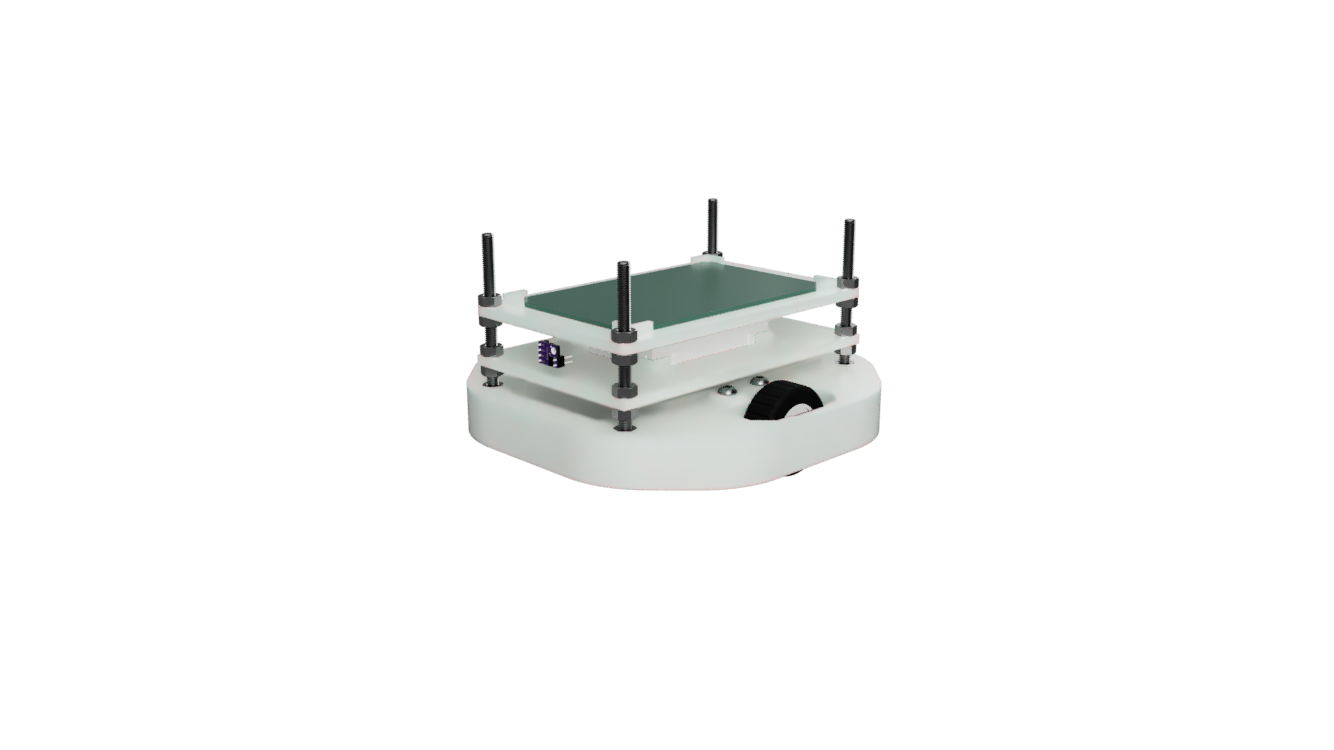
\includegraphics[width=\textwidth]{Imagenes/ArturitoMain.png}
		\caption{Modelo completo.}
		\label{fig:render_completo}
	\end{subfigure}
	\hfill
	\begin{subfigure}[b]{0.48\textwidth}
		\centering
		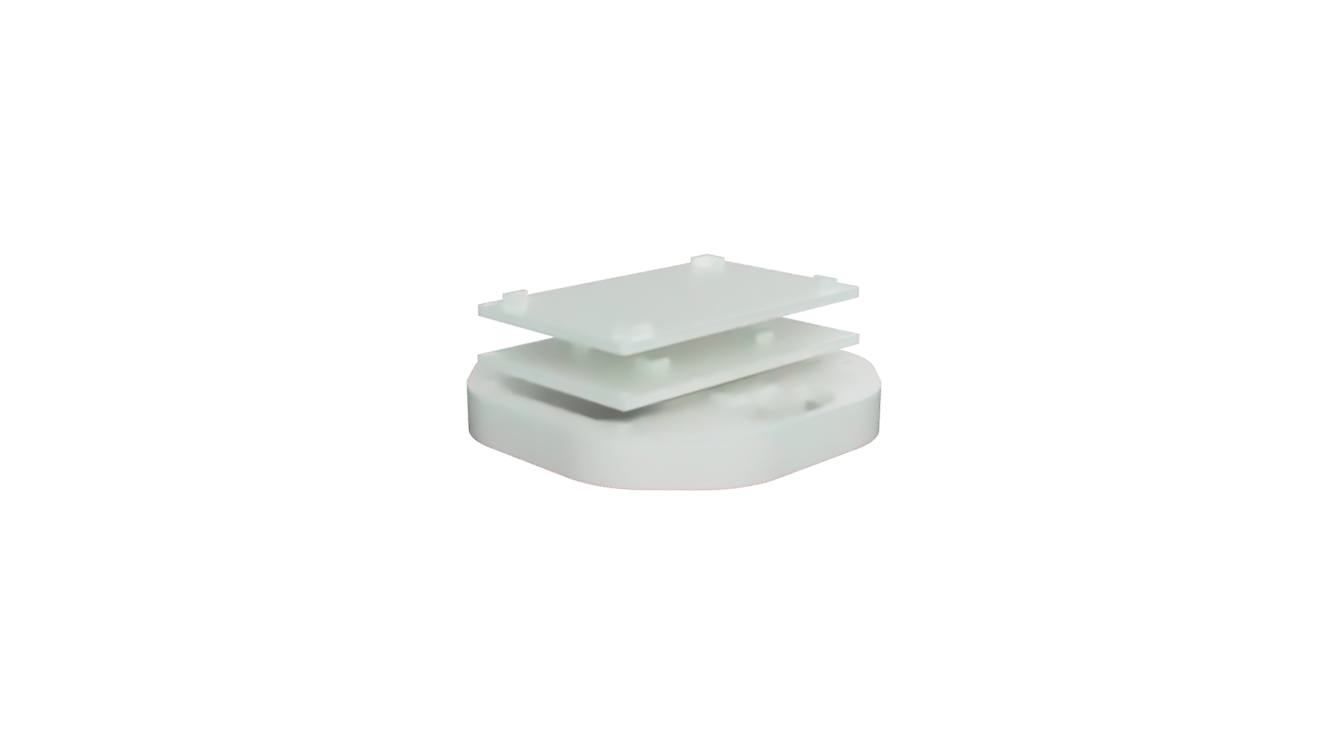
\includegraphics[width=\textwidth]{Imagenes/Impresion.png}
		\caption{Piezas impresas (ABS).}
		\label{fig:render_impresion}
	\end{subfigure}
	
	\vspace{0.3cm} % Espacio vertical entre la primera y segunda fila
	
	% --- SEGUNDA FILA: 1 imagen centrada ---
	\begin{subfigure}[b]{0.55\textwidth}
		\centering
		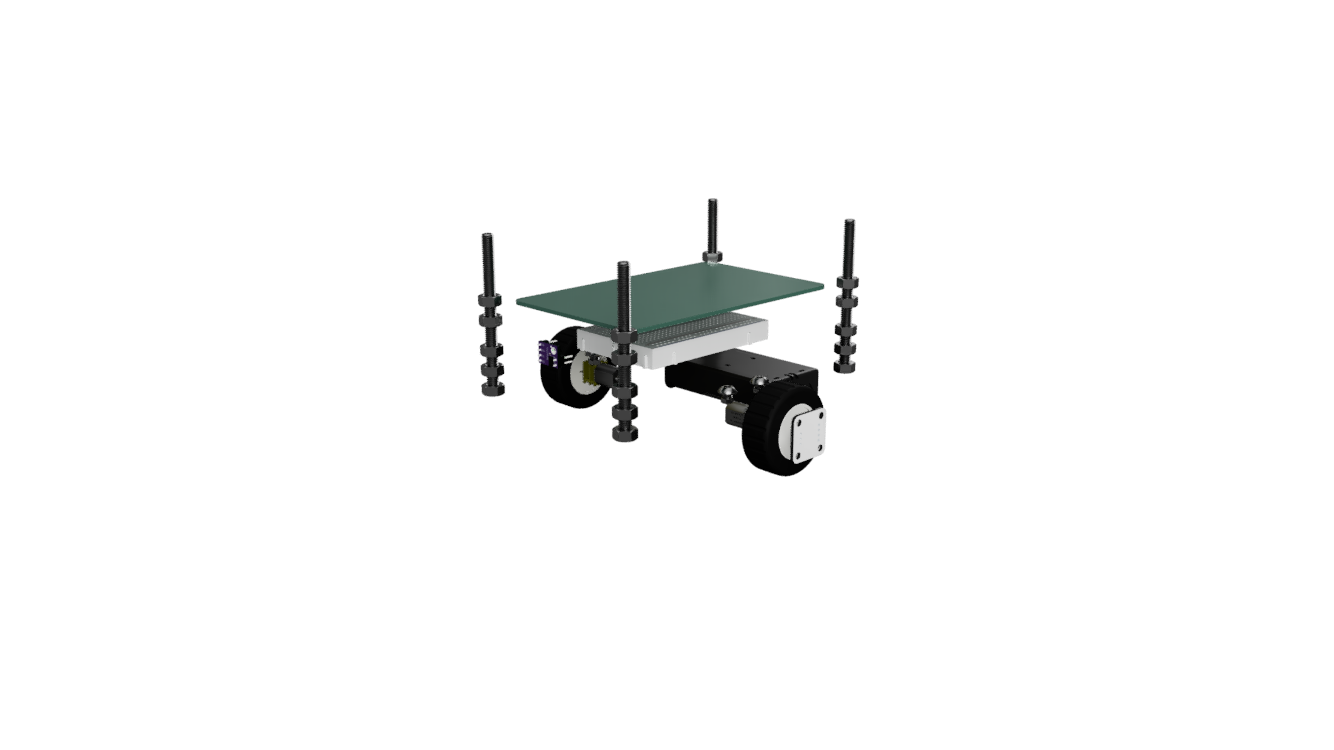
\includegraphics[width=\textwidth]{Imagenes/Referencias.png}
		\caption{Componentes/Hardware.}
		\label{fig:render_referencias}
	\end{subfigure}
	
	\caption{Desglose y vistas del modelo CAD paramétrico del chasis.}
	\label{fig:renders_chasis}
\end{figure}

\subsubsection{Arquitectura general y selección de materiales}
El chasis del robot se concibió bajo una filosofía de diseño modular y apilable en niveles, modelado de forma paramétrica en Autodesk Fusion. \pendiente{agregar el modelo CAD en un anexo o en la bibliografía.}
\begin{itemize}[nosep]
    \item \textbf{Proceso de manufactura:} impresión 3D por Fabricación por Filamento Fundido (FFF) en una impresora Creality Ender-3 S1.
    \item \textbf{Material:} ABS, por su resistencia mecánica y al impacto.
    \item \textbf{Unión de niveles:} la vinculación estructural vertical entre plataformas se resuelve mediante varillas roscadas y tuercas estandarizadas M3 y M6.
\end{itemize}

\subsubsection{Requisitos del chasis}

\pendiente{incorporar estos requisitos a la sección de requerimientos del TP1 si aún no figuran.}
\begin{itemize}[nosep]
    \item \textbf{Sensores de ángulo:} cada módulo AS5600 debe quedar enfrentado a una rueda, con el imán de magnetización diametral pegado en el eje de la rueda y alineado con su eje de rotación.
    \item \textbf{Radio de giro:} el chasis debe permitir un radio de giro nulo (girar sobre su propio eje).
    \item \textbf{Sensor ToF:} el VL53L0X debe apuntar al frente, sobre el eje de simetría del chasis, con el campo de visión despejado durante el giro del robot.
    \item \textbf{Tracción:} el chasis debe poder desplazarse con los motores y ruedas disponibles.
    \item \textbf{Alimentación:} el chasis debe tener espacio para los dos sistemas de alimentación separados: un portapilas de una celda 18650 (lógica) y uno de dos celdas 18650 (potencia).
\end{itemize}

\subsubsection{Tracción y apoyo}
El sistema adopta una configuración cinemática de tracción diferencial, con dos motores GA12-N20 acoplados a ruedas de \SI{44}{mm} de diámetro. El portapilas de dos celdas se ubica en la sección posterior, para desplazar el centro de gravedad hacia el punto de apoyo. En la versión CAD actual el apoyo trasero aún no está diseñado: será un patín deslizante integrado e impreso en ABS que se ensayará en la siguiente fase de prototipado; si las pérdidas por fricción resultan elevadas, se lo reemplazará por una rueda de bolas de acero (\emph{ball caster}).

\subsubsection{Integración de sensores}
\begin{itemize}[nosep]
    \item \textbf{Módulos AS5600:} el chasis integra soportes enfrentados a cada rueda, con los ejes de rotación alineados. El imán se monta centrado en el extremo del eje de la rueda, con una separación respecto del sensor de entre \SI{1}{mm} y \SI{2}{mm}. Como el motor GA12-N20 no tiene eje trasero accesible, el imán no puede montarse en el rotor y gira a la velocidad de la rueda ($\approx$\SI{62}{RPM}), lo que simplifica el conteo de vueltas.
    \item \textbf{Soporte del sensor ToF:} se ubica en el extremo frontal, sobre el eje de simetría del robot, para garantizar un campo de visión despejado. Su geometría se encuentra en etapa de finalización.
\end{itemize}


\begin{visar}
La cobertura de $360^\circ$ se obtiene haciendo girar el robot completo, por lo que el ángulo de cada medición proviene de la odometría (AS5600) y de la IMU. Conviene medir el desplazamiento del sensor ToF respecto del centro de giro (punto medio entre ruedas) para corregirlo en el cálculo del mapa. Dado que el robot gira apoyado en el patín, pueden producirse deslizamientos que degraden la estimación del ángulo solo con los AS5600; el giróscopo de la IMU permite compensarlo.

La resolución angular depende de la velocidad de giro $\omega$ y del tiempo de medición $T_s$ del sensor: $\Delta\theta = \omega\,T_s$. Con $T_s \approx \SI{33}{ms}$ y una muestra por grado, la velocidad máxima de giro es de $\approx 30\,^\circ/\mathrm{s}$ (una vuelta completa en $\approx\SI{12}{s}$).
\end{visar}


\subsubsection{Estado de fabricación y próximos pasos}
A la fecha de este informe, el diseño 3D se encuentra en fase de cierre en entorno CAD y aún no se inició la impresión de las piezas. Los próximos pasos son:
\begin{itemize}[nosep]
    \item \textbf{Pruebas de tolerancia:} impresión de piezas de prueba con distintas tolerancias para validar los encastres de las tuercas y varillas M3 y M6 antes de imprimir el chasis completo.
    \item \textbf{Impresión 3D e integración física:} Fabricación de los niveles y montaje de la electrónica.
    \item \textbf{Validación de Apoyo:} Evaluación experimental de la fricción del apoyo de ABS.
\end{itemize}


\section{Modelado, Control y Algoritmos de Navegación}



\subsection{Bloque de Cinemática y Control de Tracción}


\subsubsection{Modelo dinámico e Identificación de la Planta del Motor GA12-N20}
Desde el punto de vista físico, el motor DC (GA12-N20) no responde de forma instantánea a los cambios de tensión debido a la inercia del rotor y la fricción de los engranajes. A su vez, existe una relación proporcional entre el ciclo de trabajo de la señal PWM aplicada a través del puente H y la velocidad angular alcanzada en estado permanente.

Para representar este comportamiento dinámico en el dominio de Laplace, la planta se modela como un sistema de primer orden:

\[G(s) = \frac{\Omega(s)}{U(s)} = \frac{K}{\tau s + 1}\]

Donde
\begin{itemize}
	\item {$\Omega(s)$} es la velocidad angular de salida de la rueda, expresada en $[rad/s]$.
	\item {$U(s)$} es la señal de control aplicada al puente H, expresada en unidades de PWM (Duty Cycle $[0-100\%]$)
	\item {$K$} es la ganancia del sistema, expresada en $[(rad/s)/unidad PWM]$.
	\item {$\tau$} es la constante de tiempo mecánica, expresada en milisegundos $[ms]$, que representa el tiempo necesario para que la respuesta alcance el $63,2\%$ de su valor de estado permanente.
\end{itemize}

Para obtener los valores de $K$ y $\tau$ para cada rueda (izquierda y derecha) se aplica un escalón de tensión partiendo del reposo y se registra la velocidad angular en función del tiempo mediante el sensor magnético AS5600.

\paragraph{Identificación de la Ganancia $K$}
Una vez alcanzado el régimen permanente, se calcula $K$ como el cociente entre la velocidad angular alcanzada y el ciclo de trabajo definido por el escalón en U(s).

\paragraph{Identificación de la constante de tiempo $\tau$}
Se determina identificando el instante de tiempo donde $t=\tau$ tal que la velocidad angular alcanzada sea del $63,2\%$.



\subsubsection{Lazo Interno: Diseño y Sintonización de Controlador PI del Motor GA12-N20}

\paragraph{Diseño en el Dominio Continuo}~\\
Habiendo identificado la función de transferencia de la planta (motor), es posible ahora plantear un lazo cerrado por PID de la velocidad angular de un motor, y por lo tanto de la rueda correspondiente.


\begin{figure}[H]
	\centering
	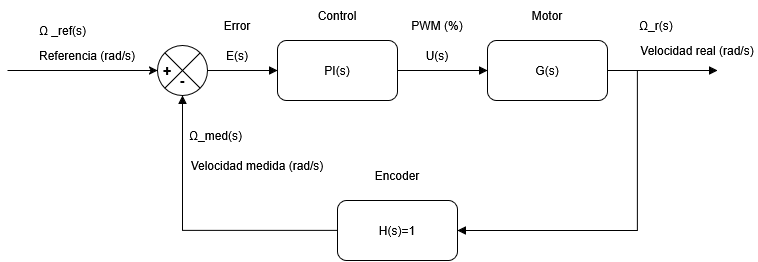
\includegraphics[width=0.8\textwidth]{Imagenes/Lazo Interno-Motor.png}
	\caption{Lazo interno de control de un motor. (MEJORAR, CAMBIAR PI POR C(S))}
	\label{fig:lazointernomotor}
\end{figure}

Donde:
\begin{itemize}
	\item {$\Omega\_$ref(s)} es la velocidad angular de referencia para el motor.
	\item {$E(s)$} es el error entre la velocidad de referencia y la velocidad medida.
	\item {$C(s)$} es el control proporcional e integral.
	\item {$U(s)$} es la señal PWM enviada al motor por $C(s)$.
	\item {$G(s)$} es la función de transferencia del motor.
	\item {$\Omega\_$r(s)} es la velocidad angular real que tiene el motor.
	\item {$H(s)=1$} es la función de transferencia del encoder, se la asume sin retrasos.
	\item {$\Omega\_$med(s)} es la velocidad medida por el encoder, utilizada para el cálculo del error.
\end{itemize}

Siendo que la función de transferencia de la planta es

\[G(s) = \frac{K}{\tau s + 1}\]

Es posible plantear un control por PI

\[C(s) = K_p + K_i/s = K_p(\frac{s+K_i/K_p}{s})\]

Donde la función de transferencia a lazo abierto es (renombrando $\tau$ como $\tau_{la}$, constante de tiempo de lazo abierto)

\[LA(s) = C(s)G(s) =  K_p(\frac{s+K_i/K_p}{s}) \frac{K}{\tau_{la} s + 1}\]

Analizando la función de lazo abierto, vemos es que posible cancelar uno de sus polos, eligiendo $K_i$ y $K_p$ tal que

\[\frac{K_i}{K_p} = \frac{1}{\tau_{la}} => K_i=\frac{K_p}{\tau_{la}}\]

Queda entonces la función de transferencia a lazo abierto

\[LA(s) = \frac{K_pK}{s\tau_{la}}\]

Al cerrar el lazo, la función de transferencia a lazo cerrado queda

\[LC(s) = \frac{LA(s)}{1+LA(s)H(s)} = \frac{\frac{K_pK}{s\tau_{la}}}{1+\frac{K_pK}{s\tau_{la}}1}\] 
\[LC(s) = \frac{1}{\frac{1}{K_pK}s+1} = \frac{1}{\tau_{lc}s+1}\]

Donde $\tau_{;c}$ es la constante de tiempo a lazo cerrado. Siendo que depende del valor de la constante $K_p$, nos da un grado de libertad para definir el tiempo de respuesta que queremos que tenga el lazo cerrado de control.

\[\tau(K_p) = \frac{1}{K_pK}\]
\[K_i(K_p) = \frac{K_p}{\tau}\]


\paragraph{Criterio del Muestreo}~\\
En el mundo real, es imposible integrar cada instante de tiempo. El intervalo de muestreo del estado del lazo cerrado (medición del sensor y computo de la lógica en consecuencia) se deberá de hacer cada cierto $\Delta t$. Para garantizar que el controlador digital represente fielmente el comportamiento diseñado en el dominio continuo, el intervalo de muestreo $\Delta t$ debe ser lo suficientemente chico respecto a la velocidad de respuesta del lazo cerrado ($\tau_{lc}$).

Un período de muestreo del orden de la constante de tiempo ($\Delta t\approx\tau_{lc}$) resulta inaceptable por: Dado que $t=\tau_{lc}$ la velocidad angular ya ha alcanzado el $63,2\%$ de su estado permanente para cuando se hace el primer muestreo. Esto impide detectar las variaciones bruscas de velocidad a lo largo del recorrido hacia el regimen permanente. Por otro lado, la aproximación de la integral por suma de rectángulos $e[k]\Delta t$ asume que el error varía suavemente entre muestras. Un $\Delta t$ elevado induce error por discretización sustancial.

Por lo tanto, se toma el criterio empírico de diseño, el cual establece que se deben tomar al menos entre 5 y 10 muestras durante la constante de lazo cerrado:

\[\Delta t <= \frac{\tau_{lc}}{10}\]

Dado que la constante de tiempo del motor a lazo cerrado es de $\tau_{lc}\approx LLENAR$, se toma entonces un valor de $\Delta t = LLENAR$.

\paragraph{Discretización}~\\
Para trasladar el lazo de control diseñado en el dominio continuo $s$ al microcontrolador, se requiere discretizar la ecuación diferencial en el dominio del tiempo t:

\[u(t)=K_pe(t)+K_i\int_{0}^{t} e(m) \,dm\]

Evaluando $t = k\Delta t$ (donde $k$ representa el número de muestra actual y $\Delta t$ el período de muestreo elegido anteriormente), se obtiene la ecuación en diferencias:

\[u[k]=K_pe[k]+\sum_{i=1}^{k} e[i]\Delta t\]

Donde la integral se aproxima mediante una suma de Riemann (rectángulos de ancho $\Delta t$ y altura $e[k]$).

El cálculo directo de la sumatoria $\sum_{i=1}^{k} e[i]\Delta t$ requeriría de almacenar todo el historial de errores en memoria RAM, lo que incrementaría el tiempo de procesamiento a medida que el robot opera.

Para resolver esto, es posible expresar la integral k-ésima de manera recursiva, en función del cálculo anterior. Siendo $I[k]$ el término integral:

\[I[k] = I[k-1] + e[k]\Delta t\]

De esta forma el algoritmo solo conserva en memoria un único valor, resultando en la ecuación en diferencias final:

\[u[k]=K_pe[k]+K_iI[k]\]

VER DE HACER EL CODIGO ACA O EN ALGUN LADO, TAMBIEN MENCIONAR QUE EN EL CODIGO SE DEBERIA LIMITAR LA SALIDA DEL CONTROLADOR PI (u(s)) A MAX 100\% y MIN 0\%.

\subsubsection{Cinemática Directa: Odometría Primaria a partir de Encoders}


\subsubsection{Lazo Externo: Control Cinemático Polar para Seguimiento Punto a Punto}


\subsubsection{Cinemática Inversa}




\subsection{Bloque de Mapeo y Estimación de Posición}


\subsubsection{Análisis Experimental de Deriva Odométrica en theta}


\subsubsection{Corrección de orientación mediante IMU}


\subsubsection{Modelado del sensor TOF y construcción de la grilla de ocupación}




\subsection{Bloque de Navegación Autónoma}


\subsubsection{Estrategia de exploración y selección de metas}


\subsubsection{Algoritmo de evasión de obstáculos}




\subsection{Integración de Lazos y Arquitectura de Control Global}


\subsubsection{Diagrame unificado del sistema de control}


\subsubsection{Máquina de estados y lógica de selección de modos}
% ==============================================================================
\newcommand{\ruta}[1]{\texttt{#1}}
% SECCIÓN 1: INTRODUCCIÓN Y JUSTIFICACIÓN ARQUITECTÓNICA
% ==============================================================================
\section{Diseño de Firmware}

El diseño del firmware para un sistema embebido robótico representa un desafío crítico: se deben ejecutar de manera concurrente tareas de control determinista en tiempo real junto con algoritmos pesados de procesamiento espacial y servicios no deterministas de comunicación inalámbrica.

Para evitar los cuellos de botella característicos de las arquitecturas tradicionales basadas en bucles secuenciales infinitos (\textit{Super-Loops}), se ha seleccionado una \textbf{Arquitectura Jerárquica en Capas} gobernada por el kernel de tiempo real \textbf{FreeRTOS} sobre la plataforma EDU-CIAA.

\subsection{Arquitectura propuesta y criterios de diseño}

El firmware se diseñará para integrar la percepción, la estimación de la pose,
la construcción del mapa y el control del rover diferencial. La arquitectura
será portable entre plataformas: el desarrollo y la validación funcional se
realizarán primero sobre ESP32/Arduino ya que no contamos con una EDU-CIAA en nuestras casas para desarrollar y probar software de aplicación; luego se portará a EDU-CIAA reutilizando la
aplicación y los drivers compartidos, y reemplazando la capa de adaptación al
hardware.

Se adopta una organización en tres capas para separar las operaciones propias
de cada placa de los algoritmos del robot. Esta separación permite probar los
módulos por partes, mantener una única implementación de la lógica del rover y
evitar que las decisiones de una placa condicionen el código común. La
arquitectura de ejecución se organizará en tareas periódicas controladas por
tiempo y planificadas por FreeRTOS, la implementación y caracteristicas de este todavia no se decidieron ya que primero optamos por validar los datos del hardware e integrarlo con una simple versión del scheduler.

El modelo elegido prioriza interfaces estables entre capas, unidades físicas
comunes y un main compartido. El período de muestreo y las prioridades se
ajustarán mediante mediciones de carga y latencia cuando se integren los
encoders, la construcción del mapa y el control de motores.

\newpage
\subsection{Las Tres Capas}

\begin{figure}[h!]
    \centering
    \includegraphics[width=1\textwidth]{imagenes/capas.png}
    \caption{Estructura jerárquica de la arquitectura en capas para el firmware de Arturito.}
    \label{fig:capas_software}
\end{figure}
\begin{description}

  \item[Capa 1 --- HAL (Hardware Abstraction Layer).]
       Será una interfaz común y tendra una implementación por placa. Su objetivo
        principal es abstraer el acceso a los periféricos y recursos de bajo
        nivel del microcontrolador, tales como GPIO, I2C, UART, PWM,
        temporizadores e interrupciones, evitando que las capas superiores
        dependan directamente de registros o características especificas de
        una arquitectura.

        Cada plataforma tendrá su propia implementación de estas funcionalidades.
        Por ejemplo, una implementación para la EDU-CIAA podrá configurar
        directamente registros del LPC4337, mientras que otra implementación
        podrá utilizar funciones provistas por sAPI o LPCOpen. De manera
        equivalente, una implementación para ESP32 podrá utilizar los drivers
        proporcionados por ESP-IDF.

        Por lo tanto, la existencia de la HAL no implica que todos los
        periféricos deban implementarse desde cero mediante acceso directo a
        registros. Si la arquitectura dispone de una biblioteca o driver que
        ya implementa dicha funcionalidad, la función correspondiente de la
        HAL podrá encapsular esa implementación. De esta manera, las capas
        superiores mantienen siempre la misma interfaz independientemente de
        cómo se resuelva internamente cada operación.

        La HAL no realizará tratamiento de las
        mediciones ni algoritmos propios del funcionamiento del rover.
        Sin embargo, en aquellos casos en que una biblioteca específica de
        una plataforma ya proporcione funciones de mayor nivel para acceder a
        un dispositivo, la HAL podrá encapsular dichas funciones con el fin de
        mantener una interfaz uniforme entre arquitecturas. En estos casos terminaria actuando como una HAL de perifericos.
        El procesamiento
        común de las mediciones continuará perteneciendo a los drivers de
        dispositivos. La HAL tampoco realizará integración de pose, mapeo ni
        navegación.

        \begin{visar}
Ejemplos de funciones HAL:
\begin{itemize}

  \item \texttt{hal\_gpio\_config()} 

  \item \texttt{hal\_gpio\_write()} 

  \item \texttt{hal\_i2c\_init()} 

  \item \texttt{hal\_i2c\_read()} 

  \item \texttt{hal\_pwm\_set\_duty()} 


  \item \texttt{hal\_imu\_get\_gyro\_z\_rads()} representa el caso en que la capa se comporta como HAL de perifericos. Si la plataforma dispone de una
        biblioteca específica para un periferico, podría encapsular directamente
        la función equivalente de dicha biblioteca. De esta forma, las capas
        superiores utilizan la misma interfaz independientemente de la
        implementación disponible en cada arquitectura.

\end{itemize}
        \end{visar}


  \item[Capa 2 --- Drivers de dispositivos.]
        Interpretará las señales físicas de cada dispositivo y entregará datos
        listos para la aplicación. Incluirá lectura, calibración, corrección y
        validación de datos de los sensores y podrá enviar comandos de
        generación de señales de control para el DRV8833. Sus interfaces no
        dependerán de Arduino ni de sAPI.

        \begin{visar}
Ejemplos de funciones de drivers:
\begin{itemize}

  \item \texttt{driver\_mpu6050\_get\_gyro\_z\_rads()}

  \item \texttt{driver\_vl53l0x\_get\_distance\_m()}

  \item \texttt{driver\_as5600\_get\_angle\_rad()} 

  \item \texttt{driver\_motor\_set\_pwm()}

  \item \texttt{driver\_motor\_set\_direction()}

\end{itemize}
        \end{visar}


  \item[Capa 3 --- Aplicación.]
        Contendrá la lógica propia del rover: adquisición y sincronización de
        muestras, cinemática diferencial y estimación de pose, actualización
        de la grilla de ocupación, selección de consignas según el modo y
        distribución de datos a la navegación y las comunicaciones. Acá
        vivirán los algoritmos de estimación de pose, mapeo y navegación.

        \begin{visar}
Ejemplos de funciones de aplicación:
\begin{itemize}

  \item \texttt{odometry\_update()} 



  \item \texttt{pose\_estimator\_update()}

  \item \texttt{occupancy\_grid\_update()} 

  \item \texttt{navigation\_update()} 

\end{itemize}
        \end{visar}


  \item[Infraestructura transversal --- FreeRTOS.]
        FreeRTOS no se considerará una capa adicional de la arquitectura, sino
        una infraestructura transversal utilizada para organizar la ejecución
        concurrente del sistema. El kernel se encargará de la planificación de
        las tareas, sus prioridades y temporización, además de proporcionar
        mecanismos de comunicación y sincronización.

        La lógica de aplicación podrá dividirse en tareas periódicas o
        activadas por eventos, por ejemplo para adquisición de sensores,
        control de velocidad, estimación de pose, actualización del mapa,
        navegación y comunicaciones. Cuando resulte necesario, los drivers y
        la HAL también podrán utilizar mecanismos proporcionados por FreeRTOS
        para sincronizar accesos a recursos compartidos.

        

\end{description}

\subsection{Software de PC e interfaz de usuario prevista}

El alcance para el programa de PC es visualizar la pose del rover y
el mapa actualizado. Para transmitir
pose y mapa sin cable se prevé incorporar Wi-Fi o Bluetooth. La elección entre ambos protocolos queda pendiente. Además desde allí se podran mandar órdenes START/STOP y, como objetivos
secundarios, teleoperación y planificación de rutas; su incorporación como
controles de esta interfaz queda por definir.

\begin{figure}[H]
    \centering
    \includegraphics[width=1\linewidth]{imagenes/InterfazDispExt.png}
    \caption{Interfaz para ver el mapeo desde el punto de vista del usuario.}
    \label{fig:interfaz-dispext}
\end{figure}

Desde esta vista se puede imaginar el siguiente ciclo: 

\begin{center}
\fbox{\parbox{0.91\linewidth}{\centering
Inicio $\rightarrow$ conexión con el rover $\rightarrow$ espera de datos
$\rightarrow$ visualización continua de pose y mapa $\rightarrow$ pérdida de
enlace: indicar desconexión / conexión restablecida: reanudar visualización}}
\end{center}

Si se pierde el enlace durante la operación, el firmware deberá aplicar la
parada segura y la interfaz indicará la desconexión. 

\subsection{Bibliotecas y herramientas externas previstas}

\begin{itemize}
  \item \textbf{ESP32:} framework Arduino y su integración con FreeRTOS;
        \texttt{Wire} para I2C; biblioteca Adafruit \texttt{VL53L0X} para el
        sensor ToF. Para el transporte inalámbrico se utilizará la capacidad
        disponible en ESP32 una vez elegido el protocolo de enlace.
        Para la compilación, carga y estructura general del sistema se utiliza PlatformIO.
  \item \textbf{EDU-CIAA:} LPCOpen y SAPI para la placa y sus periféricos, más
        el kernel FreeRTOS configurado en el proyecto. La HAL de algunos modulos estan implementados (por ejemplo: MPU60x0, el cual brinda acceso simplificado al sensor MPU6050) mientras que hay sensores como el ToF que no tienen esta libreria especifica y al cual le tendremos que desarrollar la implementación de acceso I2C por registros.

  \item \textbf{Workspace:} Se logró integrar ambos entornos de desarrollo en un mismo wokspace para VScode. 

  \begin{figure}[h!]
    \centering
    \includegraphics[width=0.3\textwidth]{imagenes/workspace.png}
    \caption{Estrucura del Workspace.}
    \label{fig:workspace}
\end{figure}
  
  \begin{description}
  \item[\ruta{docs/}] Documentos del equipo.
  \item[\ruta{shared/}] Contratos HAL, drivers y logica de aplicación que no
        deben depender de Arduino ni de sAPI.
  \item[\ruta{esp32/}] Firmware PlatformIO para ESP32, sus HAL de placa y
        programas de diagnostico independientes.
  \item[\ruta{edu-ciaa/}] Copia de estructura del entorno de 'Embedded IDE'. Make, LPCOpen, sAPI, todo lo necesario para la compilación y carga sobre EDU-CIAA. Adapta la
        misma aplicación y drivers a su arquitectura.
  \item[\ruta{processing/}] Por ahora esta carpeta es nuestra "PC externa". Contiene sketches que reciben datos para visualizar.
\end{description}
\end{itemize}


\newpage

\subsection{Estado actual y ensayos realizado}

A la versión actual de firmware la llamamos V0 (Versión 0). Esta versión ya cuenta con la estructura base del workspace explicado anteriormente pero solo realiza el siguiente ciclo de percepción:

\begin{enumerate}
  \item Inicializa la IMU MPU6050 y el sensor de distancia VL53L0X.
  \item Lee la velocidad angular del eje Z de la IMU y una distancia del ToF.
  \item Corrige e integra la velocidad angular para estimar el angulo $\theta$.
  \item Acepta distancias entre 0.05 m y 1.50 m; el resto se representa como
        $-1$ (medida invalida o sensor no disponible).
  \item Publica una linea CSV con $\theta$ en radianes y distancia en metros.
  \item Processing (programa graficador) representa la orientación y acumula puntos del ToF mientras
        el robot gira en el lugar.
\end{enumerate}

No hay todavía odometria XY, encoders, motores, navegación autónoma ni grilla de
ocupación. No hay modos de funcionamiento por comandados ni comunicación inalámbrica.

El firmware V0 fue cargado tanto en ESP32 como en EDU-CIAA y validado con Processing: se comprobó la
recepción de las muestras serie y la visualización de orientación y distancia.
\begin{figure}[h!]
    \centering
    \includegraphics[width=0.6\textwidth]{imagenes/V0.png}
    \hfill
    \includegraphics[width=0.38\textwidth]{imagenes/f1.png}
    \caption{Visualización de V0 en Processing (izquierda) y sensores montados en un auto a control remoto (derecha). \href{https://drive.google.com/file/d/1k8-xx6FHV0KANsshld4rqhePZVvpV37A/view?usp=drive_link}{Link para ver funcionamiento en video.}}
    \label{fig:v0_y_sensores}
\end{figure}

\newpage
\subsubsection{Cómo llegamos a V0}

Firmware V0 es en realidad una versión final de un proceso de testeo de los sensores en ambas arquitecturas, de un proceso de interpretación de datos, de armado de workspace, de ejecución del programa con FreeRTOS, etc.

Algunos cosas interesantes de mensionar:
\begin{description}
 \item[Angulo entregado por capa 1 vs Angulo provisto por capa 2:]
 
 La capa 2 espera que el robot quede quieto, promedia 1000 lecturas separadas por 2
ms para estimar el offset, y reinicia el estado de integración, luego resta el offset, elimina velocidades dentro de ±1◦/s, calcula un promedio trapezoidal entre muestras y acumula el angulo con el tiempo transcurrido.
   \begin{figure}[h!]
    \centering
    \includegraphics[width=0.9\textwidth]{imagenes/V0-grados.jpeg}
    \caption{Obtención del angulo crudo vs. procesado por capa 2.}
    \label{fig:grados_crudos}
\end{figure}

Se ve que a tan solo 30s de inicializado el rover el angulo crudo difiere en 5° del angulo real (el rover estaba quieto).

   \begin{figure}[h!]
    \centering
    \includegraphics[width=0.9\textwidth]{imagenes/resta.jpeg}
    \caption{Angulo procesado - Angulo crudo}
    \label{fig:resta_grados}
\end{figure}
Acá se puede ver que si se mueve el robot cambia la relacion entre una señal y la otra. Si el procesado no fuese necesario entonces este grafico deberia ser casi siempre 0 o aunque sea aproximarse a 0. 

 \item[Error en la librería de MPU para EDU-CIAA:] como ya mencionamos, existe una librería que otorga recursos para manejar el giroscopio y acelerometro MPU6050 dentro de sAPI. Durante las pruebas de integración en hardware de se identificó un error que hacia que el sensor no responda.

El procedimiento de arranque de la libreria implementaba una verificación de integridad mediante la lectura del registro interno WHO\_AM\_I (dirección 0x75), cuyo valor de retorno esperado según la hoja de datos estándar del fabricante es 0x68. Sin embargo, la función de inicialización abortaba de forma consistente retornando un código de falla (-5), impidiendo la ejecución del resto del sistema.

Tras analizar el bus de comunicación I2C mediante rutinas de escaneo, se constató que la variante física del módulo utilizado responde con el identificador 0x72 no 0x68. Entendimos que este comportamiento es habitual en hardware genéricos y para solucionar esta incompatibilidad se reestructuró la validación en el driver. La lógica fue modificada para admitir de forma flexible tanto el identificador nativo (0x68) como el valor identificado en el banco de pruebas (0x72).

\end{description}


% ==============================================================================
% SECCIÓN 4: CRONOGRAMA PRELIMINAR
% ==============================================================================
\section{Cronograma Preliminar}

\begin{tcolorbox}[colframe=green!60!black, colback=green!5!white, arc=2mm, title=\textbf{Cronograma (Google Sheets)}]
  En el siguiente enlace podrá acceder al cronograma preliminar detallado:
  \vspace{0.2cm}
  
  \textbf{Enlace:} \href{https://docs.google.com/spreadsheets/d/1GAEeQZzlFaMgwrWLOeSPeK0nOuYQg2peXEuDazYDfk4/edit?usp=sharing}{Ver Planilla de Cronograma en Google Sheets}
\end{tcolorbox}

% ==============================================================================
% SECCIÓN 5: DIVISIÓN DE TAREAS DEL GRUPO
% ==============================================================================
\section{División de Tareas del Grupo}

\begin{tcolorbox}[colframe=green!60!black, colback=green!5!white, arc=2mm, title=\textbf{División de tareas (Google Sheets)}]
  En el siguiente enlace podrá acceder a una plantilla con los módulos y requerimientos a realizar por integrante:
  \vspace{0.2cm}
  
  \textbf{Enlace:} \href{https://docs.google.com/spreadsheets/d/1GAEeQZzlFaMgwrWLOeSPeK0nOuYQg2peXEuDazYDfk4/edit?usp=sharing}{Ver Planilla de División de tareas en Google Sheets}
\end{tcolorbox}

\section{Bibliografía}

\begin{thebibliography}{99}

\bibitem{siegwart}
R. Siegwart, I. R. Nourbakhsh y D. Scaramuzza,
\textit{Introduction to Autonomous Mobile Robots}, 2.a ed.
Cambridge, MA, USA: MIT Press, 2011, cap. 3, pp. 89--108.
URL: \url{https://www.ucg.ac.me/skladiste/blog_13268/objava_56689/fajlovi/Introduction%20to%20Autonomous%20Mobile%20Robots%20book.pdf}.

\bibitem{thrun}
S. Thrun, W. Burgard y D. Fox,
\textit{Probabilistic Robotics}.
Cambridge, MA, USA: MIT Press, 2005, cap. 5, 8, 9, 10.
URL: \url{https://docs.ufpr.br/~danielsantos/ProbabilisticRobotics.pdf}.

\bibitem{lidar}
Homemade LIDAR sensor with Arduino \& Processing,
URL: \url{https://www.youtube.com/watch?v=fQ2iB7qkrUg}.

\bibitem{slam}
How to Make an Autonomous Mapping Robot Using SLAM,
URL: \url{https://www.youtube.com/watch?v=xqjVTE7QvOg}.

\bibitem{autonomo}
Autonomous Navigation playlist by MATLAB,
URL: \url{https://www.youtube.com/watch?v=Fw8JQ5Q-ZwU&list=PLn8PRpmsu08rLRGrnF-S6TyGrmcA2X7kg}.

\bibitem{drv8833}
Texas Instruments, \textit{DRV8833 Dual H-Bridge Motor Driver}, hoja de datos.

\bibitem{nano}
Arduino, \textit{Arduino Nano}, hoja de datos.

\bibitem{vl53mod}
Microcontrollers Lab, \textit{VL53L0X LIDAR Distance Sensor Interfacing with Arduino}, URL: \url{https://microcontrollerslab.com/vl53l0x-module-interfacing-arduino/}.

\bibitem{as5600mod}
TinyTronics, \textit{AS5600 Magnetic Angle Sensor Encoder Module (AS5600MOD)}, URL: \url{https://www.tinytronics.nl/en/sensors/magnetic-field/as5600-magnetic-angle-sensor-encoder-module}.

\bibitem{ga12n20}
Handson Technology, \textit{G12-N20 Geared Mini DC Motor}, hoja de datos, URL: \url{https://www.handsontec.com/dataspecs/motor_fan/GA12-N20.pdf}.

\bibitem{ciaaconsumo}
Retro-Ciaa,\textit{Lic. Santiago Germino, Biblioteca Digital, Facultad de Ingeniería, Universidad de Buenos Aires} , URL: \url{https://bibliotecadigital.fi.uba.ar/files/original/ecb2999e1e35ec2daea21bd31b3343a1.pdf}.

\bibitem{vl53l0x}
STMicroelectronics, \textit{VL53L0X: Time-of-Flight ranging sensor}, hoja de datos.

\bibitem{as5600}
ams-OSRAM, \textit{AS5600: 12-Bit Programmable Contactless Potentiometer}, hoja de datos.

\bibitem{mt3608}
Aerosemi, \textit{MT3608 2A Step-Up Converter}, hoja de datos.

\bibitem{esp32}
Espressif Systems, \textit{ESP32 Series Datasheet}.

\bibitem{ciaa}
Proyecto CIAA, \textit{EDU-CIAA-NXP}, esquemáticos y documentación.

\bibitem{kicad}
KiCad EDA, URL: \url{https://www.kicad.org/}.

\bibitem{MPU Datasheet}
MPU 6050 Datasheet, URL: \url{https://www.alldatasheet.com/datasheet-pdf/view/517744/ETC1/MPU-6050.html}.



\end{thebibliography}

% ==============================================================================
% ANEXOS / APÉNDICES
% ==============================================================================
\newpage
\section{Anexo}

\subsection{Circuito Esquemático}

\begin{figure}[H]
    \centering
    % Controla la altura máxima para no empujar el título
    \includegraphics[width=\textwidth, height=0.75\textheight, keepaspectratio]{imagenes/Esquematico.pdf}
    \caption{Esquemático completo del sistema de control y potencia.}
    \label{fig:esquematico_anexo}
\end{figure}

% ------------------------------------------------------------------------------
\subsection{Lista de materiales (BOM)}
% ------------------------------------------------------------------------------
\begin{table}[H]
\centering
\caption{Lista de materiales preliminar.}
\label{tab:bom}
\small
\begin{tabular}{cL{5.6cm}L{1.6cm}L{3cm}}
\toprule
Ítem & Descripción / código de parte & Cant. & Formato \\
\midrule
1 & Motorreductor GA12-N20 (Handson Technology), \SI{6}{V}--\SI{12}{V}, 150:1 & 2 & Motor con caja metálica \\
2 & Módulo driver DRV8833 & 1 & Módulo, pines 2,54~mm \\
3 & Módulo elevador MT3608 (\SI{5}{V}, ramal de lógica) & 1 & Módulo \\
4 & Celda Li-ion 18650, \SI{3,7}{V} (capacidad a confirmar) & 3 & Cilíndrica \\
5 & Portapilas 18650: uno de 1 celda y uno de 2 celdas en serie & 2 & Portapilas \\
6 & Protección de celdas (BMS), no definida & \pq & \pq \\
7 & Cargador de celdas, no definido & \pq & \pq \\
8 & Capacitor electrolítico \SI{470}{\micro F}/\SI{16}{V} & 1 & Componente discreto \\
9 & Capacitor cerámico \SI{100}{nF} (104) & 2 & Componente discreto \\
10 & ESP32 DevKit v1 & 1 & Módulo \\
11 & IMU MPU6050 & 1 & Módulo \\
12 & Módulo sensor de distancia VL53L0X & 1 & Módulo \\
13 & Módulo AS5600 (TinyTronics AS5600MOD), con imán diametral incluido & 2 & Módulo \SI{23}{mm}$\times$\SI{23}{mm} \\
14 & Ruedas de \SI{44}{mm} de diámetro & 2 & Rueda plástica / goma \\
\midrule
15 & Filamento ABS (para impresión 3D de piezas estructurales) & \SI{1}{kg} & Carrete de filamento \\
16 & Chasis inferior (nivel base para motores, celdas y sensores) & 1 & Pieza impresa (ABS) \\
17 & Chasis superior modular para prototipado (soporte de \emph{breadboard}) & 1 & Pieza impresa (ABS) \\
18 & Chasis superior modular (soporte para placa EDU-CIAA) & 1 & Pieza impresa (ABS) \\
19 & Varilla roscada M6 de \SI{1}{m} & 1 & Varilla \\
20 & Tuercas hexagonales M6 & 20 & Tornillería \\
21 & Tornillos M3 & 6 & Tornillería \\
22 & Tuercas hexagonales M3 & 6 & Tornillería \\
23 & Apoyo trasero: patín impreso en ABS (o \emph{ball caster} de acero) & 1 & Pieza impresa / Comp. \\
\bottomrule
\bottomrule
\end{tabular}
\end{table}
\pendiente{confirmar cantidades y qué materiales ya se poseen, como la EDU-CIAA y los motores del prototipo.}

\end{document}